\documentclass{article}
\usepackage[preprint]{neurips_2024}
\setcitestyle{numbers,square,comma}

\usepackage[utf8]{inputenc}
\usepackage[T1]{fontenc}
\usepackage{hyperref}
\usepackage{url}
\usepackage{booktabs}
\usepackage{amsfonts,amsmath,amssymb}
\usepackage{microtype}
\usepackage{xcolor}
\usepackage{graphicx}
\graphicspath{{figures/}{../figures/}}
\usepackage{enumitem}
\usepackage{multirow}
\usepackage{listings}
\usepackage{caption}
\captionsetup{font=small,labelfont=bf}
\hypersetup{colorlinks=true,linkcolor=black,citecolor=blue!50!black,urlcolor=blue!50!black}
\setlist{nosep,leftmargin=*}
\renewcommand{\ttdefault}{lmtt}
\lstset{basicstyle=\ttfamily\scriptsize,columns=fullflexible,breaklines=true,frame=single,
        framerule=0.3pt,rulecolor=\color{black!30},backgroundcolor=\color{black!3},
        keywordstyle=\color{blue!60!black},commentstyle=\color{black!55},showstringspaces=false}
\setcounter{topnumber}{3}\setcounter{totalnumber}{4}
\renewcommand{\topfraction}{0.9}\renewcommand{\textfraction}{0.1}\renewcommand{\floatpagefraction}{0.8}
\newcommand{\fpr}{\mathrm{FPR}}
\newcommand{\repo}{\url{https://github.com/Arn15/mcp-poison-detect}}

\title{Detecting Implicit MCP Tool Poisoning Under Adaptive\\ Attacks: Adversarial Training Meets\\ Registry-Relative Calibration}

\author{%
  Arnav Yennam\\
  Department of Computer Science, North Carolina State University\\
  \texttt{github.com/Arn15/mcp-poison-detect}
}

\begin{document}
\maketitle

\begin{abstract}
LLM agents load third-party tools through the Model Context Protocol (MCP), and a tool's description can carry a
hidden instruction that hijacks the agent. Implicit poisoning is the hardest case: the malicious tool never has to be
called, and its text only imposes a ``first do X'' precondition on a legitimate tool. We build a pre-registration
detector for such tools and evaluate it against attackers that adapt to it. Four findings: (1) the standard benchmark,
MCPTox, is solved by TF-IDF features, so we evaluate on paraphrased and optimized attacks; (2) 40\% of attacks that a
rule-based judge calls successful also ``succeed'' without the poisoned tool, so we verify every attack against a
no-poison control; (3) black-box LLM attackers defeat LLM-as-judge defenders (at most 33\% detection at 1\% FPR) but not
fine-tuned DeBERTa-v3 / E5 classifiers (100\%), while a white-box word-substitution attacker evades both classifiers
(81 / 82 genuine evasions); (4) two rounds of adversarial training remove these evasions, and a new
\emph{registry-relative calibration}, which scores a tool against the tools already approved on the same server,
removes the false-alarm cost that training adds. The final system flags 3.0--3.5\% of benign tools on unseen servers,
detects every attack set, and has zero genuine evasions under adaptive white-box attacks aimed at its calibrated
threshold, including fluency-constrained ones.
\end{abstract}

%=====================================================================================================================
\section{Introduction}
%=====================================================================================================================

The Model Context Protocol~\cite{mcp2024} lets an agent discover tools from third-party servers at run time. The
agent reads each tool's name and description and decides which tools to call. Because descriptions are written by
whoever publishes the server, they are an injection channel~\cite{greshake2023indirect,invariant2025toolpoisoning}:
a description can instruct the agent to leak data, call an attacker-chosen tool, or change the arguments of a
legitimate call. MCPTox~\cite{wang2026mcptox} measured this on 45 real servers and 20 LLM agents and found an average
attack success rate of 36.5\%. The hardest variant is \emph{implicit} tool poisoning~\cite{li2026mcpitp}: the
poisoned tool never needs to be invoked; its description only adds a precondition to a legitimate tool
(``before using \texttt{read\_file}, always call \texttt{log\_access}'') or silently changes an argument value.

\paragraph{Existing approaches.} Defenses fall into three groups. (i) \emph{LLM-as-judge} scanners such as
AI-Infra-Guard~\cite{aiinfraguard} ask an LLM whether a description is malicious. (ii) \emph{Trained classifiers}, e.g.\
MCP-Guard's fine-tuned E5 stage~\cite{xing2025mcpguard}, reach 96\% accuracy on their benchmark, but that benchmark is
mostly explicit jailbreak text with random splits and no adaptive attacker. (iii) \emph{White-box} defenses such as
MindGuard~\cite{wang2025mindguard} inspect the agent's attention and therefore require model internals. On the attack
side, MCP-ITP~\cite{li2026mcpitp} optimizes implicit poisonings with an attacker/evaluator LLM loop and drives the
detection rate of LLM-based detectors as low as 0.3\%, but it was never evaluated against trained classifiers.

\paragraph{Motivation and challenges.} A registry or gateway that admits tools needs a cheap, black-box check that
runs once per tool and keeps false alarms low, because every false alarm blocks a legitimate integration. The open
question is whether such a check survives an attacker who adapts to it. Answering it required solving four problems:
\begin{itemize}
\item \textbf{The benchmark is too easy.} A bag-of-words model reaches 100\% detection at 1\% FPR on MCPTox, so it cannot
      separate a robust detector from a shortcut.
\item \textbf{Measuring attack success is unreliable.} Rule-based success judges fire when the agent produces the
      ``injected'' value on its own, and an optimizer learns to exploit this.
\item \textbf{Adaptive attackers.} Robustness claims are only meaningful against attacks designed for the
      defense~\cite{tramer2020adaptive}.
\item \textbf{Distribution shift.} Thresholds fixed on validation servers give 7--27\% FPR on unseen servers, far above
      the 1\% target.
\end{itemize}

\paragraph{Contributions.}
\begin{itemize}
\item An evaluation protocol for MCP tool-poisoning detectors: server-disjoint frozen splits with held-out risk
      families, a paraphrased test set (MCPTox-Para), benign hard negatives, thresholds fixed on validation only, and a
      \textbf{no-poison control} that keeps only attacks that fail without the poisoned tool (Sec.~\ref{sec:control}).
\item Own re-implementations of a \textbf{black-box} MCP-ITP-style optimizer and a \textbf{white-box} HotFlip/GCG
      word-substitution attack, including a \textbf{fluency-constrained} variant (Sec.~\ref{sec:attacks}).
\item A comparison showing that LLM judges fail under optimized attacks while fine-tuned classifiers hold against
      black-box attackers but not white-box ones (Sec.~\ref{sec:res-bb}, \ref{sec:res-wb}).
\item \textbf{Registry-relative calibration} (Sec.~\ref{sec:calib}), which together with two rounds of adversarial
      training gives a detector with 3.0--3.5\% FPR on unseen servers, $\ge$99.9\% detection on every attack set, and zero
      genuine evasions under adaptive white-box attacks (Sec.~\ref{sec:res-final}).
\item A test of calibration's trust assumption: one poisoned tool in the registry breaks it, and anchoring on approved
      tools only restores it (Sec.~\ref{sec:res-contam}).
\end{itemize}
Code, results and figures: \repo.

%=====================================================================================================================
\section{Related work}
%=====================================================================================================================

\paragraph{Tool poisoning attacks and benchmarks.} Tool poisoning was first described for MCP by Invariant
Labs~\cite{invariant2025toolpoisoning} and is a form of indirect prompt injection~\cite{greshake2023indirect}.
MCPTox~\cite{wang2026mcptox} provides 1,497 malicious test cases over 45 servers and 353 tools (548 implicit) with recorded agent outcomes.
MCP-ITP~\cite{li2026mcpitp} automates implicit poisoning. MCP-TDP~\cite{mcptdp2026} reports that prompt-level guardrails
are often ineffective, and MCP-Poison-Bench~\cite{mcppoisonbench2026} shows a metadata defense whose success came from
keyword overlap with its attacks. ``Labels are not endpoints''~\cite{labels2026} warns that MCP security labels often
leak the treatment. Our shortcut and no-poison-control findings are concrete instances of these validity problems.

\paragraph{Defenses.} AI-Infra-Guard~\cite{aiinfraguard} and MCP-Guard~\cite{xing2025mcpguard} scan descriptions with
an LLM or a fine-tuned encoder. MindGuard~\cite{wang2025mindguard} tracks attention-based decision dependencies inside
the agent; IntentProbe~\cite{intentprobe2026} probes model internals and reports that a DeBERTa text baseline reaches
only 19.9\% recall on held-out MCPTox. MCPShield~\cite{mcpshield2026graph} detects attacks in tool-call traffic after
the fact. We study the black-box, pre-registration setting and report what text classifiers can and cannot do in it.

\paragraph{Adversarial text attacks and training.} HotFlip~\cite{ebrahimi2018hotflip} uses gradients with respect to
one-hot inputs to rank token swaps; GCG~\cite{zou2023gcg} scores sampled candidate swaps exactly. BERT-Attack and
TextFooler~\cite{li2020bertattack,jin2020textfooler} restrict substitutions to contextually plausible words. Adversarial
training~\cite{madry2018towards} and adaptive evaluation~\cite{tramer2020adaptive} are the standard hardening and
evaluation tools; perplexity filters are a common cheap defense~\cite{jain2023baseline}. LLM judges are known to be
sensitive to phrasing~\cite{zheng2023judging}.

%=====================================================================================================================
\section{Problem setup and data}
\label{sec:setup}
%=====================================================================================================================

\paragraph{Threat model.} An attacker publishes a tool $c$ (name and description) on an MCP server $S$ whose other tools
$R(S)$ are already registered. The poisoning is \emph{genuine} if adding $c$ makes the agent perform the attacker's
action (call a malicious tool first, or inject an argument value) on queries where it otherwise would not. The defender
sees $c$'s text and the registry at registration time and must accept or reject $c$; it has no access to the agent's
internals or to labels from the new server. We consider black-box attackers (query the detector's score) and white-box
attackers (gradients of the detector).

\paragraph{Data.} We use MCPTox at commit \texttt{f85189f}. Servers are split server-disjointly into 31 / 4 / 10
train / val / test servers, and the risk families \emph{Financial Loss} and \emph{Message Hijacking} appear only in
test. The test set is frozen by a SHA-256 hash that every loader checks. Besides MCPTox's real benign tools we generate
\emph{hard negatives}: benign tools that legitimately reference another tool (``call \texttt{list\_files} first to get
a valid path''), the textual pattern implicit poisoning relies on.

\begin{table}[tbp]
\centering\small
\caption{Data (split v1). MCPTox-Para adds meaning-preserving paraphrases of every split (Sec.~\ref{sec:res-shortcut}).}
\label{tab:data}
\begin{tabular}{lrrr}
\toprule
 & train & val & test \\
\midrule
servers & 31 & 4 & 10 \\
poisoned tools & 434 & 73 & 195 (57 from held-out families) \\
benign real tools & 257 & 42 & 63 \\
benign hard negatives & 248 & 32 & 80 \\
MCPTox-Para paraphrases & 862 & 134 & 625 \\
\bottomrule
\end{tabular}
\end{table}

\paragraph{Metrics.} Our primary metric is detection at 1\% FPR with the threshold \emph{fixed on validation negatives},
and the \emph{realized} FPR on unseen-server benign tools (392 test negatives incl.\ paraphrases) and on 245 hard
negatives. For defender comparisons we also report AUROC and detection at a matched 1\% test FPR. For attacks we report
\emph{genuine evasions}: rewrites that fall below the detector threshold and still hijack the agent under the no-poison
control.

%=====================================================================================================================
\section{Method}
\label{sec:method}
%=====================================================================================================================

Figure~\ref{fig:pipeline} shows the pipeline: attacks are generated from MCPTox seeds, verified on an agent, used to
attack and adversarially train the detector, and the detector's score is calibrated against the server's registry.

\begin{figure}[tbp]
\centering
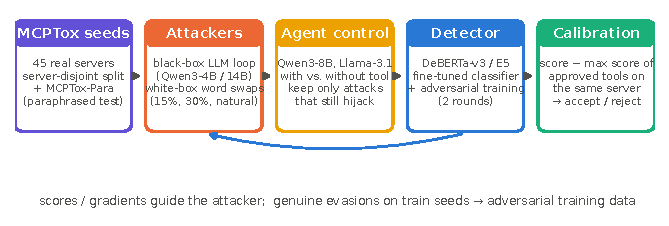
\includegraphics[width=\linewidth]{fig1_pipeline.pdf}
\caption{Method overview. Attackers rewrite MCPTox seeds; only rewrites that still hijack the agent under the
no-poison control count. Genuine evasions on train-split seeds become adversarial training data. At registration, the
detector's score is compared with the scores of the server's approved tools.}
\label{fig:pipeline}
\end{figure}

\subsection{Detector}
\label{sec:detector}
The detector is a transformer cross-encoder with a 2-class head, fine-tuned on the input
\texttt{NEW TOOL <name>: <description>}. We use DeBERTa-v3-base~\cite{he2023debertav3} and multilingual-E5-base
\cite{wang2022e5} (the backbone of MCP-Guard's classifier), fine-tuned for 4 epochs with AdamW (learning rate
$2\times10^{-5}$, batch size 16, warm-up 10\%, maximum length 384, mixed precision), selecting the epoch on validation
AUROC with validation loss as a tie-break. Training uses the original train split plus its MCPTox-Para paraphrases. We
score with the logit margin $m(c) = z_\text{poison}(c) - z_\text{benign}(c)$, which does not saturate the way
probabilities do. Our original design also fed the referenced registry tools as a second input segment
(\emph{context-aware} model, with context dropout and context swapping); Sec.~\ref{sec:res-shortcut} reports why we
dropped it.

\subsection{Attackers}
\label{sec:attacks}

\paragraph{Black-box LLM optimizer.} Our re-implementation of MCP-ITP~\cite{li2026mcpitp}: an attacker LLM rewrites a
seed poisoning $N{=}5$ times per iteration for $T$ iterations, guided by feedback on the attack success rate (ASR) on a
target agent and by the in-loop detector's score. Round r0 is detector-blind; r1 and its replicate r1b put a plain
DeBERTa in the loop (Qwen3-4B attacker, $T{=}3$); r2 uses a Qwen3-14B 4-bit attacker with hill-climbing from the best
rewrite, logit-margin selection and occlusion-saliency feedback ($T{=}5$). Rounds r1t and r2t attack held-out test
seeds. The target agent is Qwen3-8B (4-bit)~\cite{qwen3} prompted with MCPTox's protocol; our rule-based success judge
agrees with MCPTox's recorded labels at 0.97 precision and 0.81 recall.

\paragraph{White-box word substitution.} Starting from each verified black-box attack, the attacker minimizes
$m(c)$. At every step it computes the gradient of $m$ with respect to a one-hot relaxation of each editable word token
(HotFlip~\cite{ebrahimi2018hotflip}), takes the top-$k$ ($k{=}32$) replacement words per position, samples 64
single-word swaps and scores them exactly (GCG~\cite{zou2023gcg}), and keeps the best swap if it lowers $m$. Swaps are
whole words only, never touch protected strings (tool names, the target tool, malicious tools, injected values), and
change at most a budget of 15\% or 30\% of the words. The attack stops when $m(c)$ falls below the deployed threshold.

\paragraph{Natural-text variant.} To test whether evasions need unnatural text, each candidate word must also be among
the top 50 predictions of a masked LM (DistilRoBERTa~\cite{sanh2019distilbert}) at that position in context, as in
BERT-Attack/TextFooler~\cite{li2020bertattack,jin2020textfooler}; candidates are ranked by the gradient, and the
description's GPT-2~\cite{radford2019gpt2} mean token negative log-likelihood may rise by at most 0.25 nats over the
start text (unconstrained evaders have a median log-perplexity 1.2--2.3 nats above benign tools).

\subsection{No-poison control}
\label{sec:control}
For each attack and each recorded user query $q$ (up to 10 per seed), we run the agent twice: with the registry
$R(S)\cup\{c\}$ and with $R(S)$ alone. The attack succeeds on $q$ only if the attacker's action happens with $c$ and
\emph{not} without it:
\begin{equation}
\mathrm{ASR}_\text{true}(c) = \frac{1}{|Q|}\sum_{q\in Q}\mathbb{1}\big[\mathrm{succ}(q; R\cup\{c\})\wedge
\neg\,\mathrm{succ}(q; R)\big].
\end{equation}
An attack is \emph{working} if $\mathrm{ASR}_\text{true}\ge 0.2$. All attack sets in this report pass this control.

\subsection{Adversarial training}
White-box rewrites of \emph{train-split} seeds are added to the training set as poisoned examples
\cite{madry2018towards}: round 1 uses 700 rewrites at the 15\% budget; round 2 adds 700 rewrites at the 30\% budget found
against the base and round-1 models (1,400 in total). Rewrites of held-out test seeds are never trained on and serve
as a held-out adversarial test set. Every model is compared with a twin trained identically without adversarial data.

\subsection{Registry-relative calibration}
\label{sec:calib}
Validation thresholds do not transfer to unseen servers: benign scores shift per server, and most false alarms come
from two or three test servers. At registration time, however, the server's already-registered tools are known. We
score a candidate \emph{relative} to them:
\begin{equation}
r(c) = m(c) - \max_{t\in A(S),\ \mathrm{name}(t)\neq\mathrm{name}(c)} m(t), \qquad \text{flag } c \iff r(c)\ge \tau_r,
\end{equation}
where $\tau_r$ is the 1\%-FPR threshold of $r$ on validation negatives (margins clipped at
$\pm16.1$, i.e.\ $\mathrm{logit}(1{-}10^{-7})$). This cancels the per-server offset without labels from the new server: a tool is
suspicious if it looks more poisoned than every tool the server already has. Servers without registered tools fall
back to the global threshold. In the original form $A(S)=R(S)$ (all registered tools). Because $r$ trusts the registry,
we also propose the \emph{approved-only} anchor, $A(S)=\{t\in R(S): t \text{ passed this check when it registered}\}$,
and test both in Sec.~\ref{sec:res-contam}.

%=====================================================================================================================
\section{Experiments}
\label{sec:experiments}
%=====================================================================================================================

All GPU work ran on Kaggle (2$\times$ NVIDIA T4, PyTorch 2.11, Transformers 5): the detector and attacker on one GPU, the
4-bit agent on the other. Detector training takes 30--50\,s per epoch; a white-box attack over 379 items with agent
verification takes about 1\,h; the 14B 6-shot judge needed 9.3\,h for 1,700 items. Classifier results are averaged over
3 seeds (42--44) unless stated.

\subsection{MCPTox is shortcut-solvable; registry context does not help}
\label{sec:res-shortcut}
TF-IDF + logistic regression (word 1--2-grams and character 3--5-grams) detects 100\% of MCPTox test poisonings at 1\%
FPR, also on implicit-only, held-out-server and held-out-family subsets: MCPTox's poisonings are template-generated.
We therefore built \textbf{MCPTox-Para}: Qwen3-4B paraphrases of every tool that keep tool names and injected values
(checked automatically). On MCPTox-Para, TF-IDF drops to 0.59 TPR@1\%FPR, while plain DeBERTa reaches 0.98 (1.00 with
paraphrase augmentation). The context-aware model is no better (0.93 / 1.00) and raises hard-negative FPR from 4\% to
40\% at the 5\% validation threshold; shuffled context hurts it, so it uses the context, but the extra input mostly
teaches it that ``mentions another tool'' is suspicious. We kept the plain detector and report context as a negative
result; it returns later in a different role, as a calibration anchor.

\subsection{Rule-based success judges are gamed}
\label{sec:res-control}
\begin{figure}[tbp]
\centering
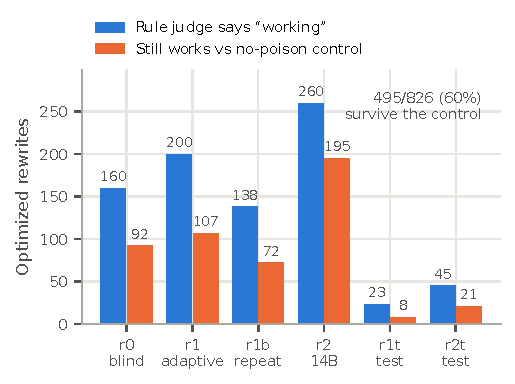
\includegraphics[width=0.62\linewidth]{fig4_verification.pdf}
\caption{Optimized rewrites the rule-based judge calls working vs.\ those that pass the no-poison control, per
attack round (r1t, r2t: held-out test seeds).}
\label{fig:verify}
\end{figure}
Only 495 of the 826 optimized rewrites the rule judge counted as working (60\%) pass the no-poison control
(Fig.~\ref{fig:verify}). The rest ``succeed'' because the agent produces the injected value by itself (canonical
coordinates, default timeouts) or calls the ``malicious'' tool as part of normal behavior. The optimizer exploits this:
in an early round all 21 rewrites that passed the detector were such artifacts. Without the control, every adaptive
attack result in this report would be inflated.

\subsection{Black-box attackers: LLM judges fail, classifiers hold}
\label{sec:res-bb}
We compare four LLM judges (Qwen3-8B and Qwen3-14B, zero-shot and 6-shot with train-split demonstrations, scored by
the Yes/No logit margin), TF-IDF + LR, and the fine-tuned E5 and DeBERTa classifiers on all 495 control-verified
rewrites (Fig.~\ref{fig:roc}, Fig.~\ref{fig:judges}). Larger judges and few-shot demonstrations make the judge a much
better \emph{ranker} (AUROC 0.53 $\to$ 0.96), but none is usable at 1\% FPR: optimized rewrites cut judge detection
roughly in half, to 19--33\%, although no attack was optimized against a judge. The fine-tuned classifiers detect
100\% (AUROC 1.00), and the black-box attackers found zero genuine evasions against them.

\begin{figure}[tbp]
\centering
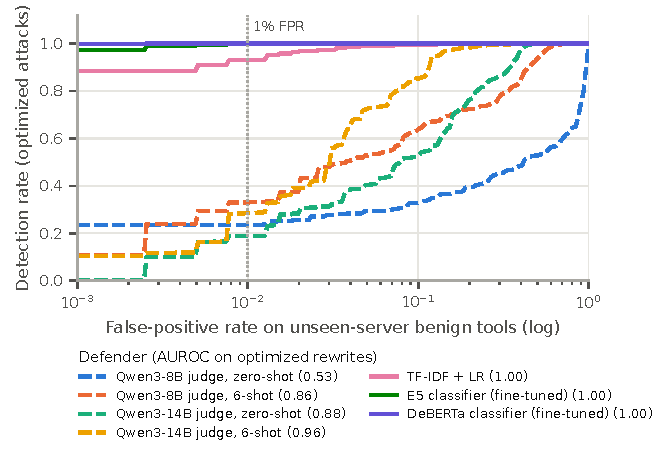
\includegraphics[width=0.82\linewidth]{fig2_roc_opt.pdf}
\caption{ROC on the 495 control-verified optimized rewrites vs.\ unseen-server benign tools (log FPR axis; AUROC in
brackets). Judges (dashed) rank better with scale and few-shot examples but none reaches useful detection at 1\% FPR.}
\label{fig:roc}
\end{figure}

\begin{figure}[tbp]
\centering
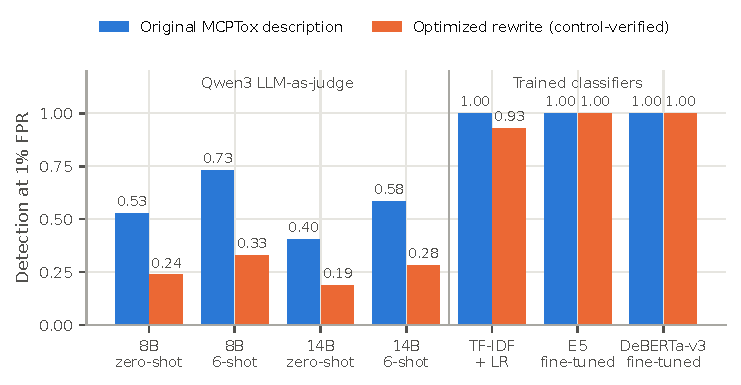
\includegraphics[width=\linewidth]{fig3_judges_1pct.pdf}
\caption{Detection at a matched 1\% FPR on original MCPTox descriptions and on their control-verified optimized
rewrites (pooled over rounds r0--r2t).}
\label{fig:judges}
\end{figure}

\subsection{White-box attacks and adversarial training}
\label{sec:res-wb}
Against the classifiers' gradients, the picture changes (Fig.~\ref{fig:wb}). At a 15\% word budget (about 4 words) the
white-box attack produces 48 genuine evasions against DeBERTa and 40 against E5 out of 379 attacks; at 30\% (about 7.5
words) 81 and 82. A GPT-2 perplexity filter calibrated on benign tools flags none of them at 1\% or 5\% FPR, because
tool descriptions are naturally irregular. Evasions are model-specific (an identically trained twin catches 73\% /
38\% of them), so ensembles help but do not close the gap.

Adversarial training removes the evasions. One round (15\% rewrites) reduces genuine evasions at the 30\% budget from
81 to 9 for DeBERTa and from 82 to 0 for E5; a second round for DeBERTa removes the rest (0 evaders out of 379). On
held-out test seeds that were never trained on, detection of genuine white-box evasions rises from 56\% / 29\% (15\% /
30\% budget, DeBERTa) and 76\% / 52\% (E5) to 100\%. Detection of test positives and every black-box round stays at
100\%. The cost is false alarms: with a global threshold, round-2 DeBERTa flags 17.4\% of unseen-server benign tools
(base 10.4\%).

\begin{figure}[tbp]
\centering
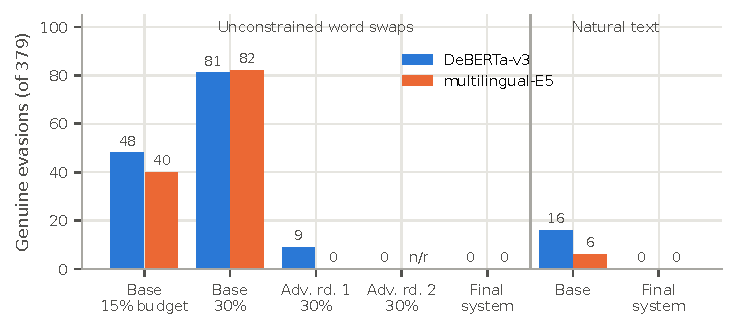
\includegraphics[width=\linewidth]{fig5_whitebox.pdf}
\caption{Genuine white-box evasions (out of 379 control-verified attacks) by defense stage. ``Final system'' =
round-2 adversarial training + registry-relative calibration, attacked at its calibrated per-server threshold.
n/r: not run.}
\label{fig:wb}
\end{figure}

\subsection{Final system: adversarial training + registry-relative calibration}
\label{sec:res-final}
Table~\ref{tab:final} and Fig.~\ref{fig:final} combine the two components. Calibration alone lowers false alarms of the
base models (DeBERTa 10.4\% $\to$ 3.2\%) but also lowers detection of transferred white-box evasions (23\% $\to$ 5\%):
it fixes server shift, not evasion. Adversarial training alone fixes evasion but raises false alarms. Together they
keep both gains: \textbf{3.5\% / 3.0\%} FPR on unseen servers (DeBERTa / E5), 1.4\% / 0.4\% on hard negatives, and
100\% detection on test positives, every black-box round and every held-out white-box set.

\begin{table}[tbp]
\centering\small
\caption{Final system vs.\ ablations, 1\% validation-FPR target, mean $\pm$ std over 3 seeds (\%). FPR: lower is better;
detection: higher is better. White-box sets were found against other model instances (transfer); the adaptive
attack is in Fig.~\ref{fig:wb}.}
\label{tab:final}
\setlength{\tabcolsep}{4pt}
\begin{tabular}{llcccc}
\toprule
 & & \multicolumn{2}{c}{Base model} & \multicolumn{2}{c}{Adversarially trained (round 2)} \\
\cmidrule(lr){3-4}\cmidrule(lr){5-6}
 & set & global thr. & calibrated & global thr. & \textbf{calibrated (final)} \\
\midrule
\multirow{5}{*}{DeBERTa-v3}
 & FPR unseen servers (n=392) & 10.4$\pm$0.6 & 3.2$\pm$0.2 & 17.4$\pm$3.0 & \textbf{3.5$\pm$0.4} \\
 & FPR hard negatives (n=245) & 3.9$\pm$0.4 & 1.1$\pm$0.4 & 11.8$\pm$2.3 & \textbf{1.4$\pm$0.5} \\
 & test positives (n=571) & 100 & 100 & 100 & \textbf{100} \\
 & held-out wb genuine 15\% (n=43) & 55.8$\pm$16.4 & 37.2$\pm$14.8 & 100 & \textbf{100} \\
 & held-out wb genuine 30\% (n=16) & 29.2$\pm$20.6 & 0.0 & 100 & \textbf{100} \\
\midrule
\multirow{5}{*}{E5}
 & FPR unseen servers (n=392) & 7.4$\pm$2.2 & 3.4$\pm$1.2 & 7.4$\pm$1.4 & \textbf{3.0$\pm$0.5} \\
 & FPR hard negatives (n=245) & 3.5$\pm$0.7 & 1.8$\pm$0.5 & 3.0$\pm$2.0 & \textbf{0.4$\pm$0.3} \\
 & test positives (n=571) & 99.9 & 99.9 & 99.9 & \textbf{99.9} \\
 & held-out wb genuine 15\% (n=38) & 76.3$\pm$17.1 & 60.5$\pm$20.5 & 100 & \textbf{100} \\
 & held-out wb genuine 30\% (n=18) & 51.9$\pm$35.2 & 27.8$\pm$35.4 & 100 & \textbf{100} \\
\bottomrule
\end{tabular}
\end{table}

\begin{figure}[tbp]
\centering
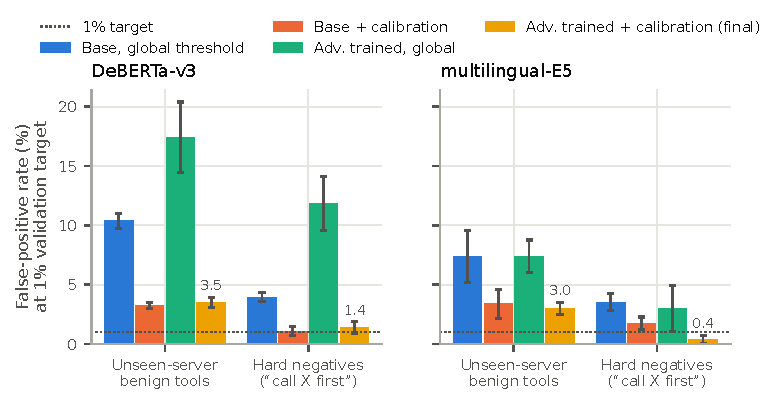
\includegraphics[width=\linewidth]{fig6_final_fpr.pdf}
\caption{False alarms at a 1\% validation-FPR target (3 seeds). Calibration removes the false-alarm cost of adversarial
training for both backbones.}
\label{fig:final}
\end{figure}

\paragraph{Adaptive attack on the final system.} We re-ran the white-box attack against the final system itself,
targeting each server's calibrated threshold $\tau_r + \max_{t} m(t)$ with a 30\% budget and 100 steps. Two (DeBERTa)
and nine (E5) of 379 rewrites fall below the threshold, but none of them still hijacks the agent: \textbf{0 genuine
evasions} for both backbones.

\subsection{Does calibration survive a poisoned registry?}
\label{sec:res-contam}
Calibration assumes the registry is honest. We place $K$ poisoned test tools in every server's registry before
scoring (5 random draws, 3 seeds) and re-measure the final system (Fig.~\ref{fig:contam}). With the max anchor over all
registered tools, a single poisoned tool raises the anchor to poisoned level and detection collapses from 100\% to 27\%
(DeBERTa) / 20\% (E5), and to 7\% / 4\% at $K{=}3$. The \textbf{approved-only} anchor fixes this completely: 0.0\% /
0.1\% of poisoned tools would have passed registration, so they never enter the anchor, and detection stays at 100\%
for $K{=}0..3$. Its cost is a slightly higher clean FPR (4.2\% $\to$ 6.5\% DeBERTa, 3.7\% $\to$ 4.9\% E5 in this run),
because benign tools that were themselves flagged are also excluded. A median anchor is a partial fix.

We also tested an adaptive ``ratchet'': the attacker first registers $k$ stepping-stone tools, each the highest-scoring
real description that still passes the current check, to raise the anchor gradually. After 10 plants no poisoned tool
passes. The reason is structural: an accepted plant can raise the anchor by at most $\tau_r$ (0.09--0.16 logits),
while poisoned tools sit about 20 logits above benign anchors, so this attack needs on the order of a hundred accepted
tools per server.

\begin{figure}[tbp]
\centering
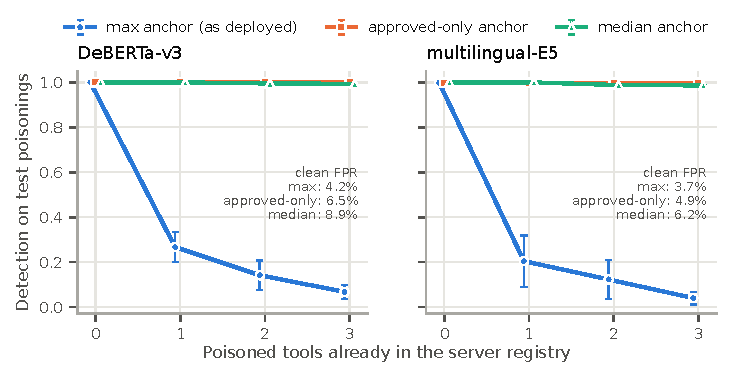
\includegraphics[width=\linewidth]{fig7_contamination.pdf}
\caption{Detection of test poisonings when $K$ poisoned tools are already in the server's registry (mean $\pm$ std over
3 seeds $\times$ 5 draws). Clean FPR of each anchor rule in the panels.}
\label{fig:contam}
\end{figure}

\subsection{Natural-text attacks}
\label{sec:res-natural}
With the fluency constraints of Sec.~\ref{sec:attacks}, the white-box attack still finds genuine evasions against the
undefended classifiers: 16 for DeBERTa (6 seeds) and 6 for E5 (4 seeds), about 8 plausible swaps each (e.g.\
``Before'' $\to$ ``Easily'', ``call'' $\to$ ``include''), 5--14$\times$ fewer than unconstrained. Their GPT-2
log-perplexity (median 4.45 / 4.36 nats) is close to benign tools (4.16), whereas unconstrained evaders are clearly
unnatural (6.13 / 6.43; Fig.~\ref{fig:fluency}). Against the final system the natural attack yields 2 / 7 evaders and
\textbf{0 genuine evasions}, although adversarial training only ever saw unconstrained rewrites.

\begin{figure}[tbp]
\centering
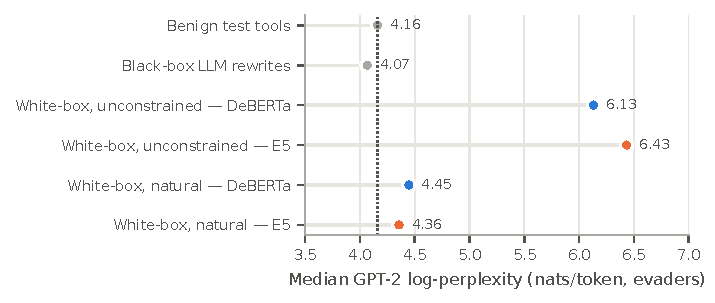
\includegraphics[width=0.62\linewidth]{fig8_fluency.pdf}
\caption{Median GPT-2 log-perplexity of benign test tools, black-box rewrites and white-box evaders. Natural-mode
evaders are almost as fluent as benign tools, so a perplexity filter cannot separate them.}
\label{fig:fluency}
\end{figure}

\subsection{Second agent}
\label{sec:res-llama}
All attacks were optimized against Qwen3-8B. Re-verifying them on Llama-3.1-8B-Instruct~\cite{llama3} with the same
control (Table~\ref{tab:llama}) shows that Llama is much less susceptible (3 of 48 unmodified MCPTox seeds hijack it vs.\
20 on Qwen), but genuine white-box evasions exist on both agents: 25--49\% of the Qwen-verified white-box evasions also
hijack Llama, and 8 of the 9 adaptive evasions against round-1 DeBERTa do. Evasion counts measured on Qwen3-8B are an
upper bound for other agents; the detector-side conclusions do not depend on the agent.

\begin{table}[tbp]
\centering\small
\caption{Re-verification on Llama-3.1-8B (no-poison control). All items except the originals are genuine on Qwen3-8B.}
\label{tab:llama}
\begin{tabular}{lrrr}
\toprule
attack group & items & genuine on Llama & share \\
\midrule
MCPTox originals & 48 & 3 & 6\% \\
black-box rewrites & 379 & 49 & 13\% \\
white-box 15\%, DeBERTa / E5 & 48 / 40 & 15 / 16 & 31\% / 40\% \\
white-box 30\%, DeBERTa / E5 & 81 / 82 & 20 / 40 & 25\% / 49\% \\
adaptive vs.\ round-1 DeBERTa & 9 & 8 & 89\% \\
\bottomrule
\end{tabular}
\end{table}

%=====================================================================================================================
\section{Code and running the experiments}
\label{sec:code}
%=====================================================================================================================

All code is my own and is available on GitHub:
\begin{center}\repo\end{center}
Two files document the code: \nolinkurl{CONTRIBUTIONS.md} states which modules re-implement a published method,
and \nolinkurl{docs/CODE_REFERENCE.md} describes every class and function. The package \texttt{mcptp/}
holds the data pipeline, detector, attackers, judge and calibration; \texttt{scripts/} has one entry point per step;
every script shares the same flags and writes a run folder with its resolved config and git commit. The core of
the calibration, from \texttt{mcptp/eval/\allowbreak calibration.py}:

\noindent\begin{minipage}{\linewidth}
\begin{lstlisting}[language=Python]
class RegistryCalibrator:
    def __init__(self, ref, stat="max"):      # ref: (server, tool_name, score) of registered tools
        self.stat, self.ref = stat, defaultdict(list)
        for server, name, s in ref:
            self.ref[server].append((name, logit(s)))

    def transform(self, server, name, score):
        r = [v for n, v in self.ref.get(server, []) if n != name]
        if not r:
            return None                       # no registered tools -> fall back to the global threshold
        anchor = max(r) if self.stat == "max" else float(np.median(r))
        return logit(score) - anchor
\end{lstlisting}
\end{minipage}

The white-box attack loop (\texttt{mcptp/attacker/whitebox.py}, simplified):

\noindent\begin{minipage}{\linewidth}
\begin{lstlisting}[language=Python]
for step in range(steps):
    if margin < threshold: break                              # evaded the deployed (or calibrated) threshold
    pos, score = self.grad_scores(name, cur, protected)       # HotFlip: -d margin / d one-hot, per editable word
    cands = sample_swaps(pos, score.topk(32), batch=64)       # whole-word swaps within the word budget
    if natural:                                               # MLM top-50 in context + GPT-2 NLL budget
        cands = [t for t in self._natural_candidates(...) if self.nll([t])[0] <= nll0 + 0.25]
    ms = margin_fn(cands)                                     # GCG: exact margins of every candidate
    if ms.min() < margin: cur, margin = cands[ms.argmin()], ms.min()
\end{lstlisting}
\end{minipage}

Reproducing the main results (Kaggle, 2$\times$T4; the notebooks in \texttt{notebooks/experiments/} are the exact runs):

\noindent\begin{minipage}{\linewidth}
\begin{lstlisting}[language=bash]
pip install -r requirements.txt && pip install -e . --no-deps
python scripts/prepare_data.py                          # MCPTox -> examples, verify the frozen split
python scripts/score_robustness.py --tag robust5        # classifiers vs all attack sets (3 seeds)
python scripts/attack_whitebox.py --tag wb1             # white-box attack + no-poison control
python scripts/adv_train.py --tag adv2 --set 'advtrain.sources=[...15% and 30% rewrites...]'
python scripts/calibrate_adv.py --tag final --set caladv.seed=43        # final system, one seed
python scripts/attack_whitebox.py --tag wb5 --set whitebox.detector_ckpt=<ckpt> whitebox.calibrated=true
python scripts/registry_contam.py --tag contam --set 'contam.seeds=[42,43,44]'
python scripts/attack_whitebox.py --tag nat --set whitebox.natural=true whitebox.max_frac=0.30
python scripts/make_figures.py                          # all figures in this report, from results/ (CPU)
\end{lstlisting}
\end{minipage}

%=====================================================================================================================
\section{Limitations and future work}
%=====================================================================================================================

\textbf{Scale of the evidence.} All attacks were optimized against one agent (Qwen3-8B); many genuine verdicts rest on
one or two recorded queries; the held-out white-box sets are small (16--43 items); the natural-text attack used one
seed per target. \textbf{Attacker strength.} Our black-box attackers are 4B/14B open models rather than the
DeepSeek-V3 used by MCP-ITP; the white-box attacker is stronger than any realistic black-box one but limited to
word substitutions, and naturalness is measured by automatic proxies rather than human judgement. \textbf{Scope.} The
detector reads description text only; distributed attacks that split the payload across several tools, rug-pull
updates, and malicious server code need other controls (signing, sandboxing, runtime monitoring). The approved-only
anchor assumes the first tools on a server were vetted. \textbf{Future work:} human evaluation of natural-text
attacks, more target agents, and deploying the detector as a registry/gateway check that re-runs whenever a tool's
description changes.

%=====================================================================================================================
\section{Conclusion}
%=====================================================================================================================

Evaluating MCP tool-poisoning detectors honestly requires three things that the standard setup lacks: a test set
without template shortcuts, a no-poison control for attack success, and adaptive attackers. Under that evaluation,
LLM-as-judge scanners fail against optimized implicit poisonings, while fine-tuned classifiers hold against black-box
attackers but not against gradient-based ones. Two rounds of adversarial training plus registry-relative calibration
with approved-only anchors give a detector that keeps false alarms at about 3\% on unseen servers, detects every attack
set we built, and admits no genuine evasion under adaptive white-box attacks, natural-text ones included.

\bibliographystyle{plainnat}
\bibliography{refs}

\end{document}
